\section{Dropping Policies}
\label{sec:policies}

Our goal with enabling partial monitoring is to allow for a specified overhead target or budget to be met while maximizing the amount of monitoring performed.
This is done by dynamically dropping a portion of the monitoring operations. In this section, we discuss in detail how this dropping decision is
made. Specifically, we first discuss how to measure the run-time monitoring
overheads and when monitoring events need to be dropped in
Section~\ref{sec:policies.slack}. Next, we investigate trade-offs created by
selecting which events are dropped. Different policies in determining which
events can be dropped create a trade-off between how closely the overhead
budget is met and the monitoring coverage achieved.

\subsection{Measuring Monitoring Overheads}
\label{sec:policies.slack}

% Slack
\begin{figure}
  \begin{center}
    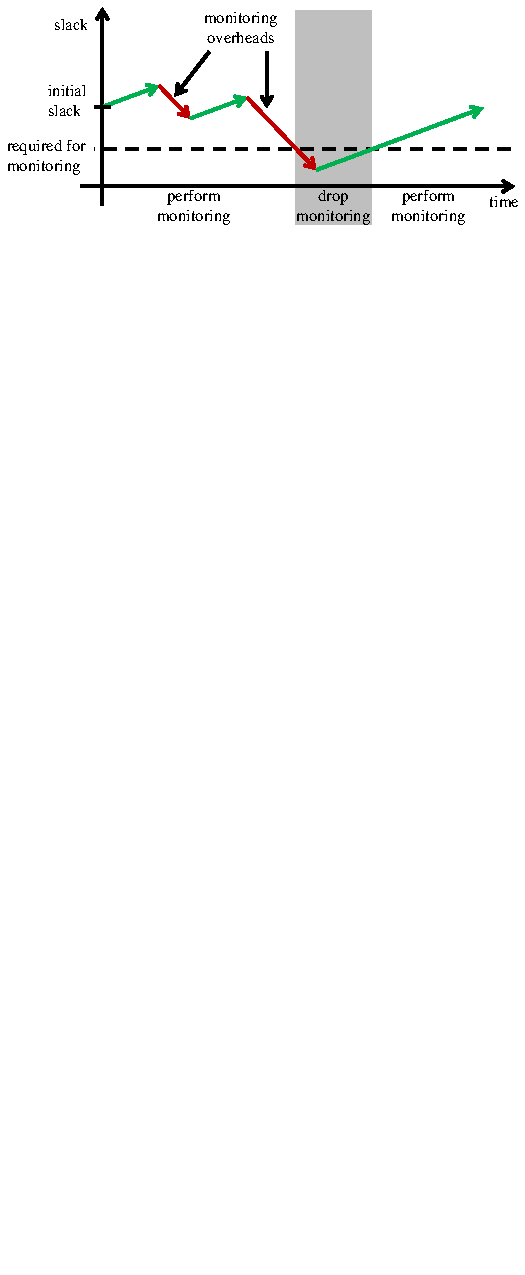
\includegraphics[width=\columnwidth]{figs/slack.pdf}
    \vspace{-0.3in}
    \caption{Slack and its effect on monitoring over time.}
    \label{fig:policies.slack}
    \vspace{-0.1in}
  \end{center}
\end{figure}

% Slack tracking module
\begin{figure}
  \begin{center}
    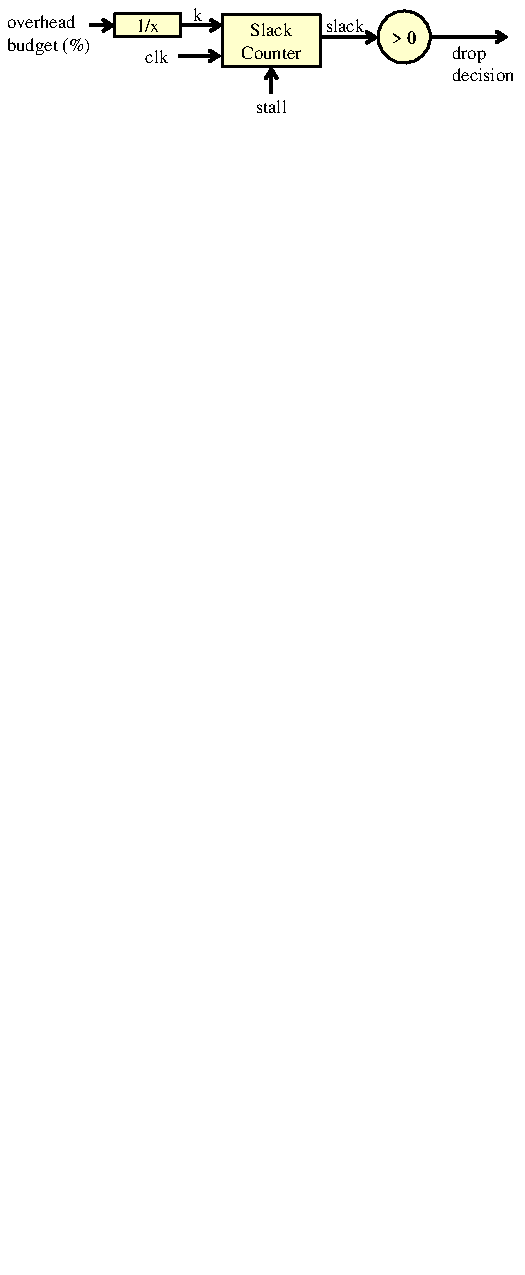
\includegraphics[width=\columnwidth]{figs/stm.pdf}
    \vspace{-0.2in}
    \caption{Slack tracking and drop decision hardware.}
    \label{fig:policies.stm}
    \vspace{-0.1in}
  \end{center}
\end{figure}

In order to decide whether a monitoring event should be dropped or not, we need
a way to keep track of overheads. In this section, we present a specific method
for measuring execution time overheads. However, we note that other methods
could be used in order to target budgets on IPC, power, energy, etc.  
% For example, one way to measure execution time overheads would be to insert
% checkpoints in the program. By recording the execution time of these
% checkpoints without monitoring, the overheads incurred while running with
% monitoring could be determined. Although this would give an accurate
% measurement of overheads, it would require modifying the program binary. In
% addition, the overhead budget for monitoring would only be updated at
% checkpoints.

% Instead, we develop a model to estimate the execution time overhead budget in a
% gradual manner and without the need to modify the main program. Specifically,
We specify the overhead budget as a percentage of the main program's execution
cycles without monitoring. We define \emph{slack} as the number of cycles of
monitoring overhead that can be incurred while staying within the budget
target. Slack is essentially the difference between the actual overheads seen
and the budget specified. Slack is generated as the main program runs and consumed as monitoring overheads occur.  For
example, if no monitoring overheads occur during 1000 cycles of the main
program's execution and the designer sets a 20\% overhead target, then the
slack that is built up during this period is 200 cycles. If the main core is
then stalled for 50 cycles due to monitoring, then the remaining slack is 150
cycles. 
In addition to this accumulated slack, a small amount of initial slack
can be given in order for monitoring to be performed at the start of a program.
Figure~\ref{fig:policies.slack} shows an example of how slack can change over time.
If the slack falls below zero (i.e., the overhead budget is exceeded), then
monitoring events should be dropped.

Figure~\ref{fig:policies.stm} shows a hardware slack tracking module for
keeping track of slack. The slack tracking module uses a counter that increments on every $k$-th
cycle of the main core. This $k$ can be calculated by taking the reciprocal of
the target budget. For example, if the target budget is 20\%, then the counter
increments on every 5th clock cycle. The value of this counter is the
accumulated slack. Whenever the main core is stalled due to the monitor, slack
is decremented. This can be difficult to determine precisely due to difficult
to measure overheads such as contention for shared memory. However, we have
found that using only the stalls due to FIFO back pressure works well in
practice.

\subsection{Dropping Decision Trade-Offs}
\label{sec:policies.events}

% Varying slack's impact on coverage for UMC
\begin{figure}
  \begin{center}
    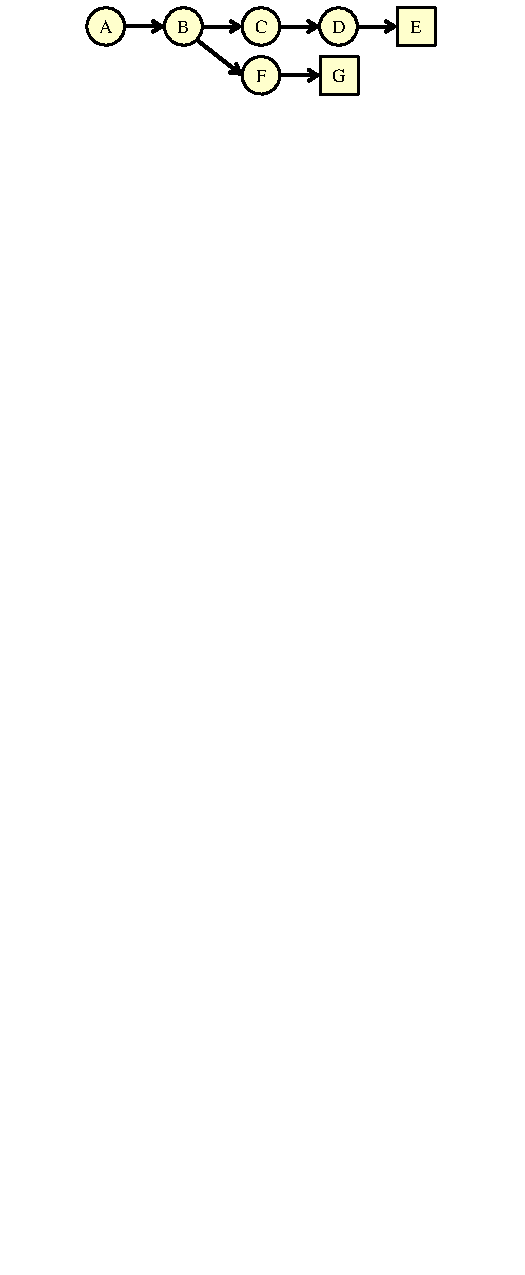
\includegraphics[width=\columnwidth]{figs/dataflow_graph.pdf}
    \vspace{-0.3in}
    \caption{Example dependence graph for metadata. Square nodes represent
    events where checks are performed.} 
    \label{fig:policies.dataflow_graph}
    \vspace{-0.1in}
  \end{center}
\end{figure}

The simplest policy for when to drop monitoring events is to drop all monitoring events as
long as slack is less than or equal to zero.  However, this can result in
wasted work. For example, consider the metadata dependence graph shown in
Figure~\ref{fig:policies.dataflow_graph}. Here, an edge from node {\tt A} to node
{\tt B} represents that if event {\tt A} is dropped, then due to its
invalidated metadata, it will cause event {\tt B} to be filtered. Square
nodes indicate events where monitoring checks are performed. In the
example, suppose that event {\tt E} is meant to perform a check operation but is dropped.
In this situation, the
monitoring operations that were done for events {\tt C} and {\tt D} were wasted
since their results were not used for any monitoring checks.

\begin{figure}
  \begin{center}
  \subfloat[unrestricted dropping]{
    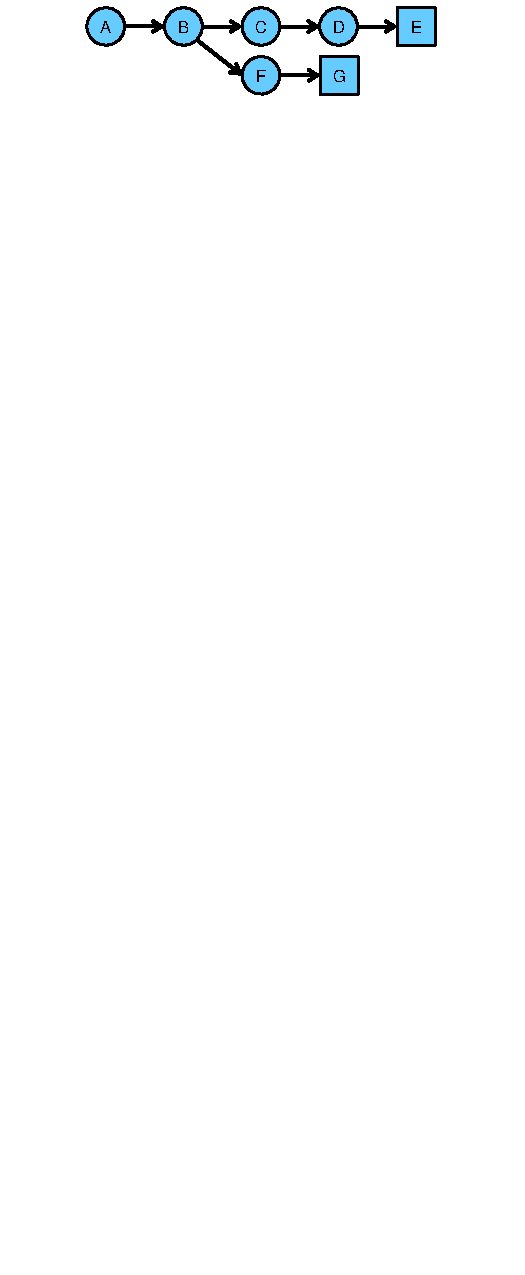
\includegraphics[width=\columnwidth]{figs/all_drop.pdf}
    \label{fig:policies.all_drop}
  }
  \vspace{-0.1in}
  \\
  \subfloat[source-only dropping]{
    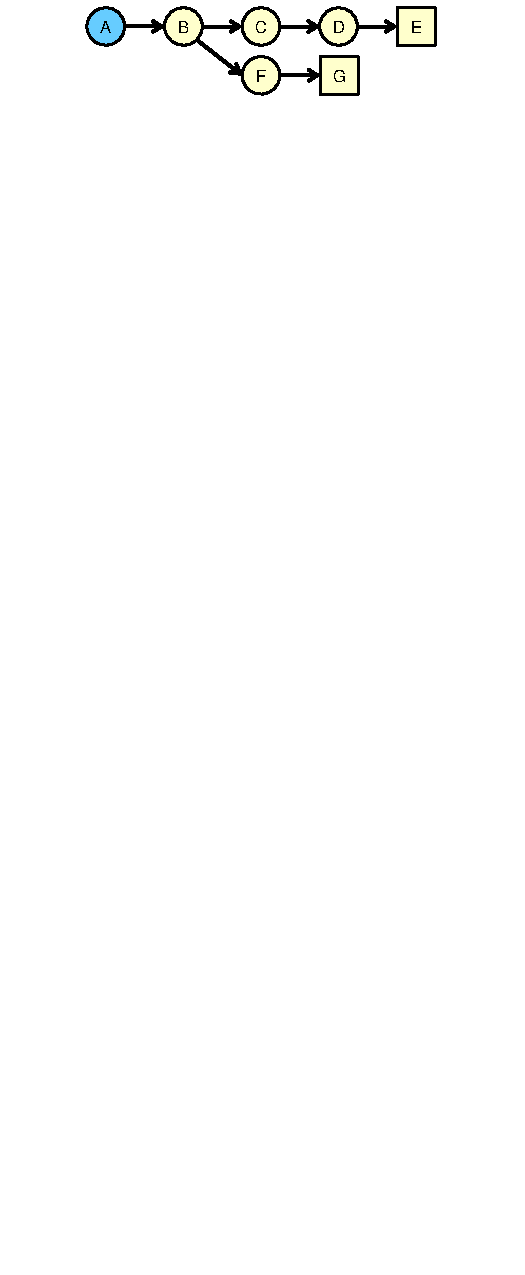
\includegraphics[width=\columnwidth]{figs/source_drop.pdf}
    \label{fig:policies.source_drop}
  }
  \vspace{-0.1in}
%   \\
%   \subfloat[sub-flow dropping]{
%     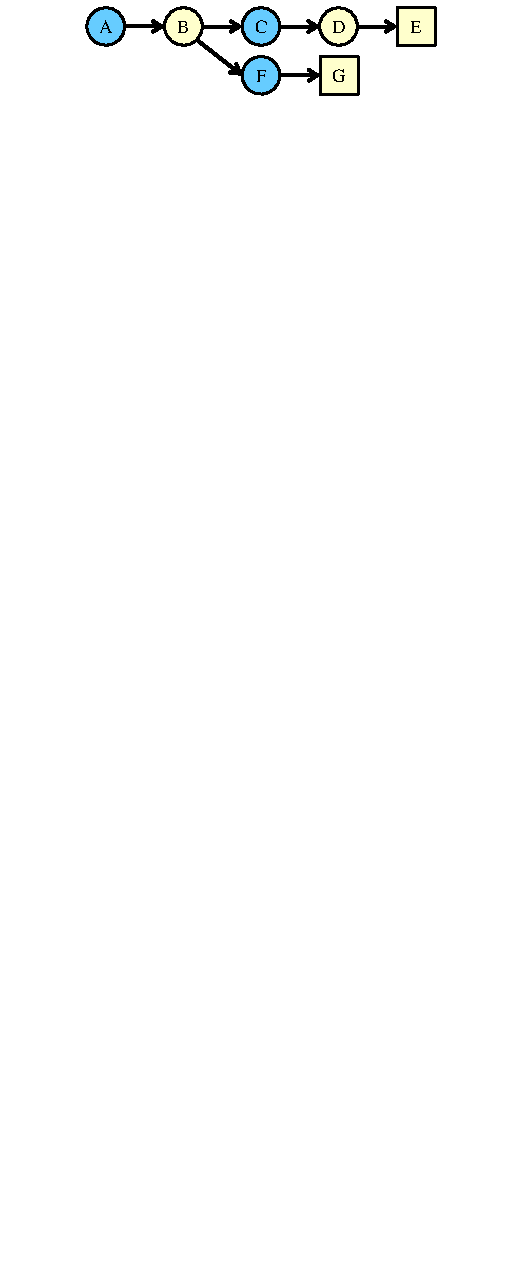
\includegraphics[width=\columnwidth]{figs/min_drop.pdf}
%     \label{fig:policies.min_drop}
%   }
  \end{center}
  \vspace{-0.1in}
  \caption{Comparison of dropping policies. Blue (dark) nodes indicate where
  dropping decisions are made.}
  \label{fig:policies.policies}
\end{figure}

One method to eliminate this wasted work is to only make dropping decisions at
the root of these metadata flows. That is, we will decide to either monitor or
not monitor an entire metadata flow. We refer to this dropping decision policy
as \emph{source-only dropping} and we refer to the previous policy of 
dropping any event as \emph{unrestricted dropping}.
Figures~\ref{fig:policies.all_drop} and \ref{fig:policies.source_drop} show a
comparison of where dropping decisions are made for these two policies. Source
dropping will
result in no wasted work and thus better coverage. However, because of the coarser-grained decision, it
may be more difficult to closely match overheads. Source dropping is expected
to work well when there are a large number of independent metadata flows.

% Trade-off between source-drop and unrestricted dropping
% \begin{figure}
%   \begin{center}
%     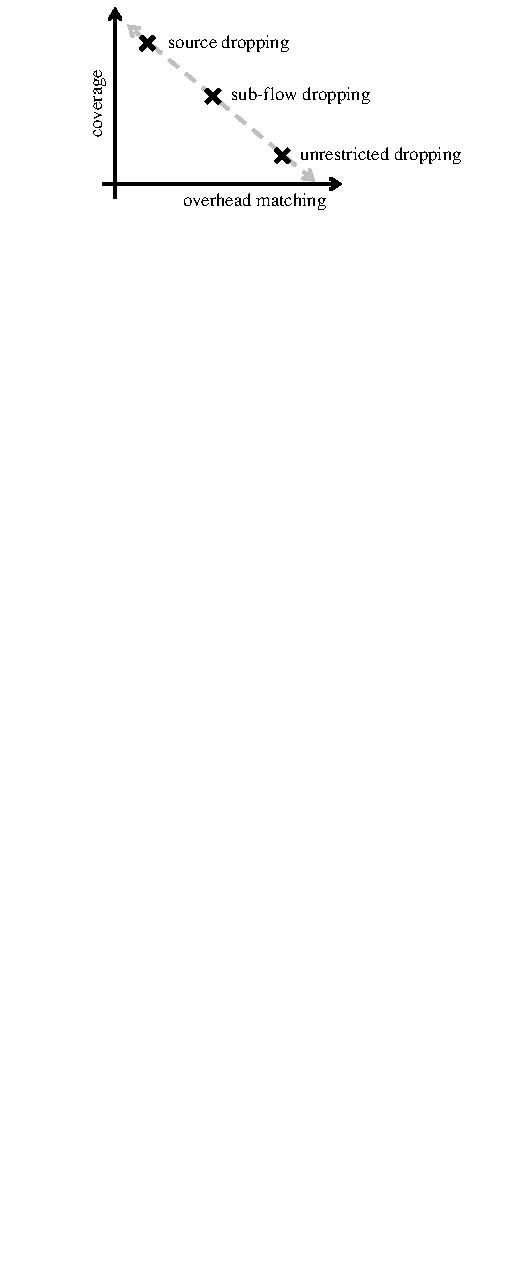
\includegraphics[width=\columnwidth]{figs/policy_trade_off.pdf}
%     \vspace{-0.3in}
%     \caption{Slack tracking and drop decision hardware.}
%     \label{fig:policies.trade_off}
%     \vspace{-0.2in}
%   \end{center}
% \end{figure}
% 
% Another possible method is to make the dropping decisions somewhere in between
% source-only dropping and unrestricted dropping. From the graph in 
% Figure~\ref{fig:policies.dataflow_graph}, we can see that if the dropping
% decision is made at event {\tt C} then we can skip event {\tt E} with no wasted
% work. If we instead choose to perform monitoring for event {\tt C}, then we want to perform all
% monitoring on that flow. Similarly, event {\tt F} creates a decision point for
% the bottom flow that will result in no wasted work and dropping event {\tt A}
% allows the entire shown metadata flow to be dropped with no wasted work. If the
% program can be
% analyzed or profiled to identify these instructions which, if dropped, lead to
% no wasted work, then this information can be used at run-time to minimize the
% amount of wasted work. We refer to this policy as \emph{sub-flow dropping}.
% Figure~\ref{fig:policies.min_drop} shows the points were dropping decisions are
% made for this policy.
% Sub-flow dropping is a coarser-grained decision than unrestricted dropping, but
% finer-grained that source-only dropping. Thus, its ability to match overheads is
% expected to sit between these other two policies. Similarly, there still exists
% edge cases where wasted work can occur, but typically we expect much less
% wasted work than unrestricted 
% dropping. Thus, we expect the coverage achieved by sub-flow dropping for a
% certain overhead to fall between source-only and unrestricted dropping. These three
% dropping policies create a trade-off space between coverage achieved and
% ability to match an overhead target.
% Figure~\ref{fig:policies.trade_off} summarizes this trade-off between coverage
% and ability to match overhead.
